%======================================================================
\chapter{Modeling 2-DOF Helicopters}
\label{ch: Chapter2}
%======================================================================
The 2-DOF helicopter, Quanser Aero [manufactured by Quanser Inc. (\href{https://www.quanser.com/}{https://www.quanser.com/})], used in the current work can be configured as a dual-rotor helicopter that has a fixed base. 
\begin{figure}[!htbp]
    \centering
    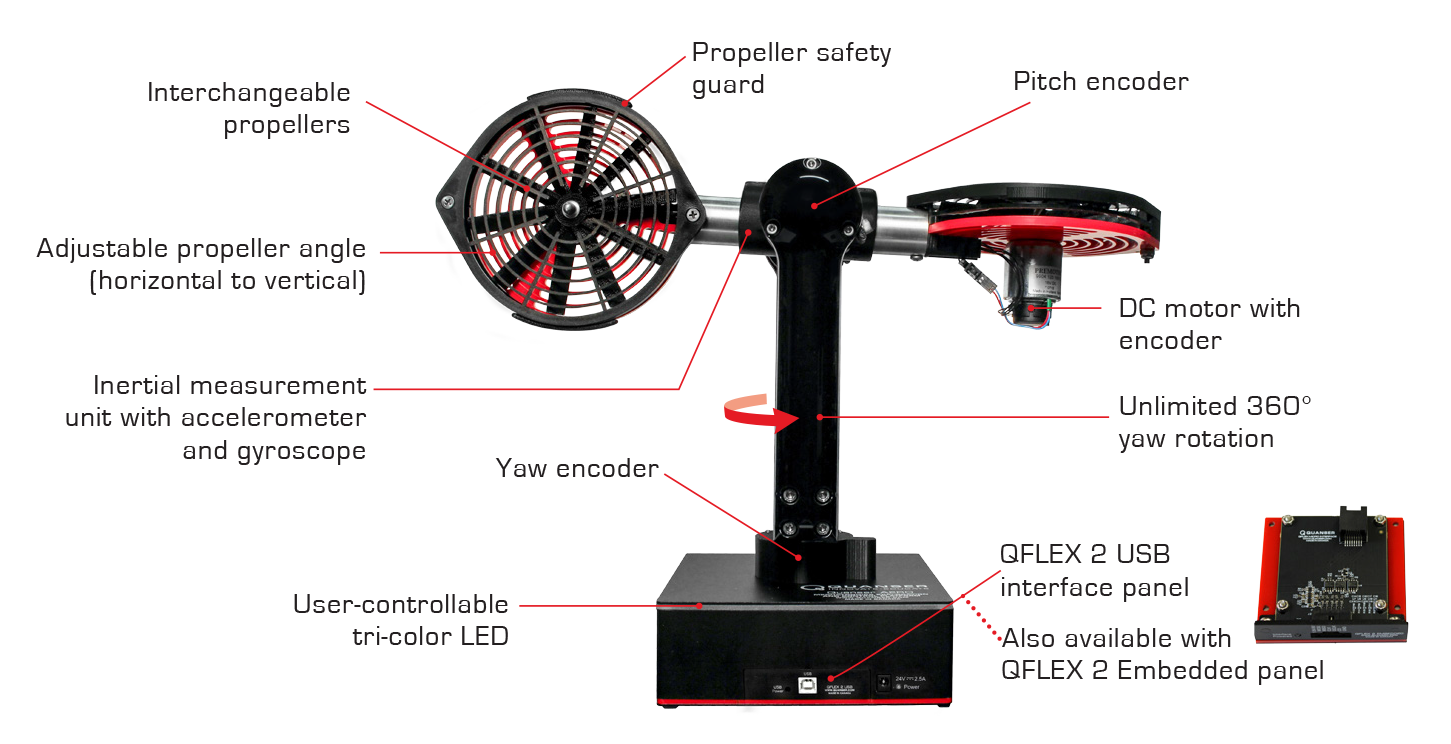
\includegraphics[width=.75\textwidth,keepaspectratio=true]{figs/img/quanserAero.png}
    \caption{The Quanser Aero 2-DOF used for experiments in the project.}
    \label{fig:quanserAero}
\end{figure}
The front rotor (horizontal to the ground) is configured to rotate about pitch axis and the tail rotor (parallel to vertical plane) is mounted to rotate about yaw axis. To measure the pitch $(\theta)$ and yaw $(\psi)$ angles, two position sensors (encoders) are mounted as shown in Fig.~\ref{fig:quanserAero}. For sake of simplicity in modeling 2-DOF helicopter, the  dynamic coupling of the Quanser Aero is omitted due to high-efficiency rotors mounted on it\footnote{See Quanser Aero user manual for details.}. The main (tail) rotor is attached to the horizontal (vertical) propeller, which is rotated by applying input voltages to corresponding DC motors. Let $v_p(v_y)$ denote the input voltage to pitch (yaw) DC motor and the state of the 2-DOF helicopter at time $t\ge 0$ is denoted by ${\bf x}^T(t) \equiv [\theta(t),\psi(t),\dot\theta(t),\dot\psi(t)],$ where $\dot\theta(\dot\psi)$ denote the rotational speed of the pitch (yaw). The free-body diagram of the 2-DOF helicopter is shown in Fig.~\ref{fig:helicopterModel}, 

\begin{figure}[!htbp]
 \begin{center}
  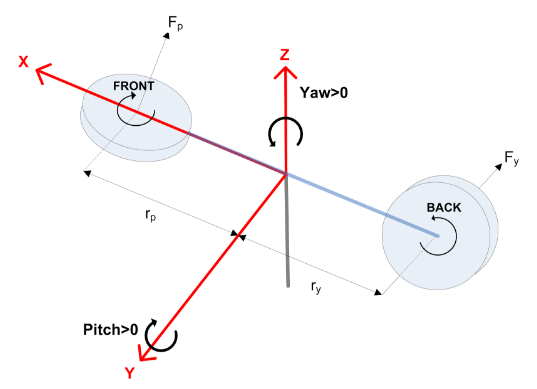
\includegraphics[scale=.75]{figs/img/helicopterModel.png}
 \end{center}
 \caption{Freebody diagram of the forces exerted on a 2-DOF helicopter.}
 \label{fig:helicopterModel}
\end{figure}

where $F_p(F_y)$ is force from the pitch (yaw) motor. If ${\bf u}^T(t)  \equiv [v_p(t),v_y(t)]$ denote the vector of the input voltages for DC motors at time $t\ge 0,$ then the state-space model of the 2-DOF helicopter (Quanser Aero) is described by~\cite{FaBiMi2018-c1}:
%
\begin{align}
  \dot{\bf x}(t) = {\bf A}{\bf x}(t) +{\bf B}{\bf u}(t),~\mathrm{where}
\label{eq:stateModel}
\end{align}  
%
\begin{align*}
{\bf A} =  
\begin{bmatrix}
0 & 0 & 1 & 0\\
0 & 0 & 0 & 1\\
-\frac{K_{\text{sp}}}{J_p} & 0 & -\frac{D_p}{J_p} &  0\\
0 & 0 & 0 & -\frac{D_y}{J_y}    
\end{bmatrix}
~\text{and}~
  {\bf B} =
\begin{bmatrix}
0 & 0\\
0 & 0\\
\frac{K_{\text{pp}}}{J_p} & \frac{K_{\text{py}}}{J_p}\\
\frac{K_{\text{yp}}}{J_y} & \frac{K_{\text{yy}}}{J_y}                           
\end{bmatrix},
\end{align*}
%
with $K_{sp},$ $K_{pp},$ $K_{py},$ $K_{yp},$ $K_{yy},$ $J_p,$ $J_y,$ $D_p,$ and $D_y$ being the stiffness of the axes, pitch motor thrust constant, thrust constant acting on the pitch angle from the yaw motor, thrust constant acting on yaw angle from pitch motor, yaw motor thrust constant, moment of inertia about pitch axis, moment of inertia about yaw axis, viscous damping of the pitch axis, and viscous damping of the yaw axis, respectively.\\ 
\\
In the context of a teleoperation system, a standard problem in controlling motion of states of a 2-DOF helicopter is to find optimal actuator commands $\mathbf{u}^*(t)\equiv[v_p^*(t),v_y^*(t)]^T,$ such that it follows the command signal, which is the desired (reference) state ${\bf x}^{d} = [\theta^{d},\psi^{d},0,0]^T,$ sent by the human operator through a mobile device. 




%----------------------------------------------------------------------
%\section{New Section}
%----------------------------------------------------------------------


%%% Local Variables:
%%% mode: latex
%%% TeX-master: "../finalReportMainV1"
%%% End:
